\begin{frame}
\begin{center}
\Huge Four \textcolor{mygreen}{Statistical methods} to analyze the results
\end{center}
\end{frame}
%------------------------------------------------

% Sensitivity analysis ------------------------------------------------
% Looking closely at the probability density of the HCL and Dong et al. equations, we see how
% similar both shapes are. These two functions estimate the avoided damage considering the cost of mitigation, 
% which drives the result. The VSL and Dechezleprêtre
% et al. avoided damage account for the indirect impact of air pollution on GDP but
% do not account for the direct cost of mitigation. If considered, the damage through
% these equations will be much higher.
\begin{frame}
    \frametitle{Sensitivity analysis}
    \begin{figure}[htb!]
        \centering
        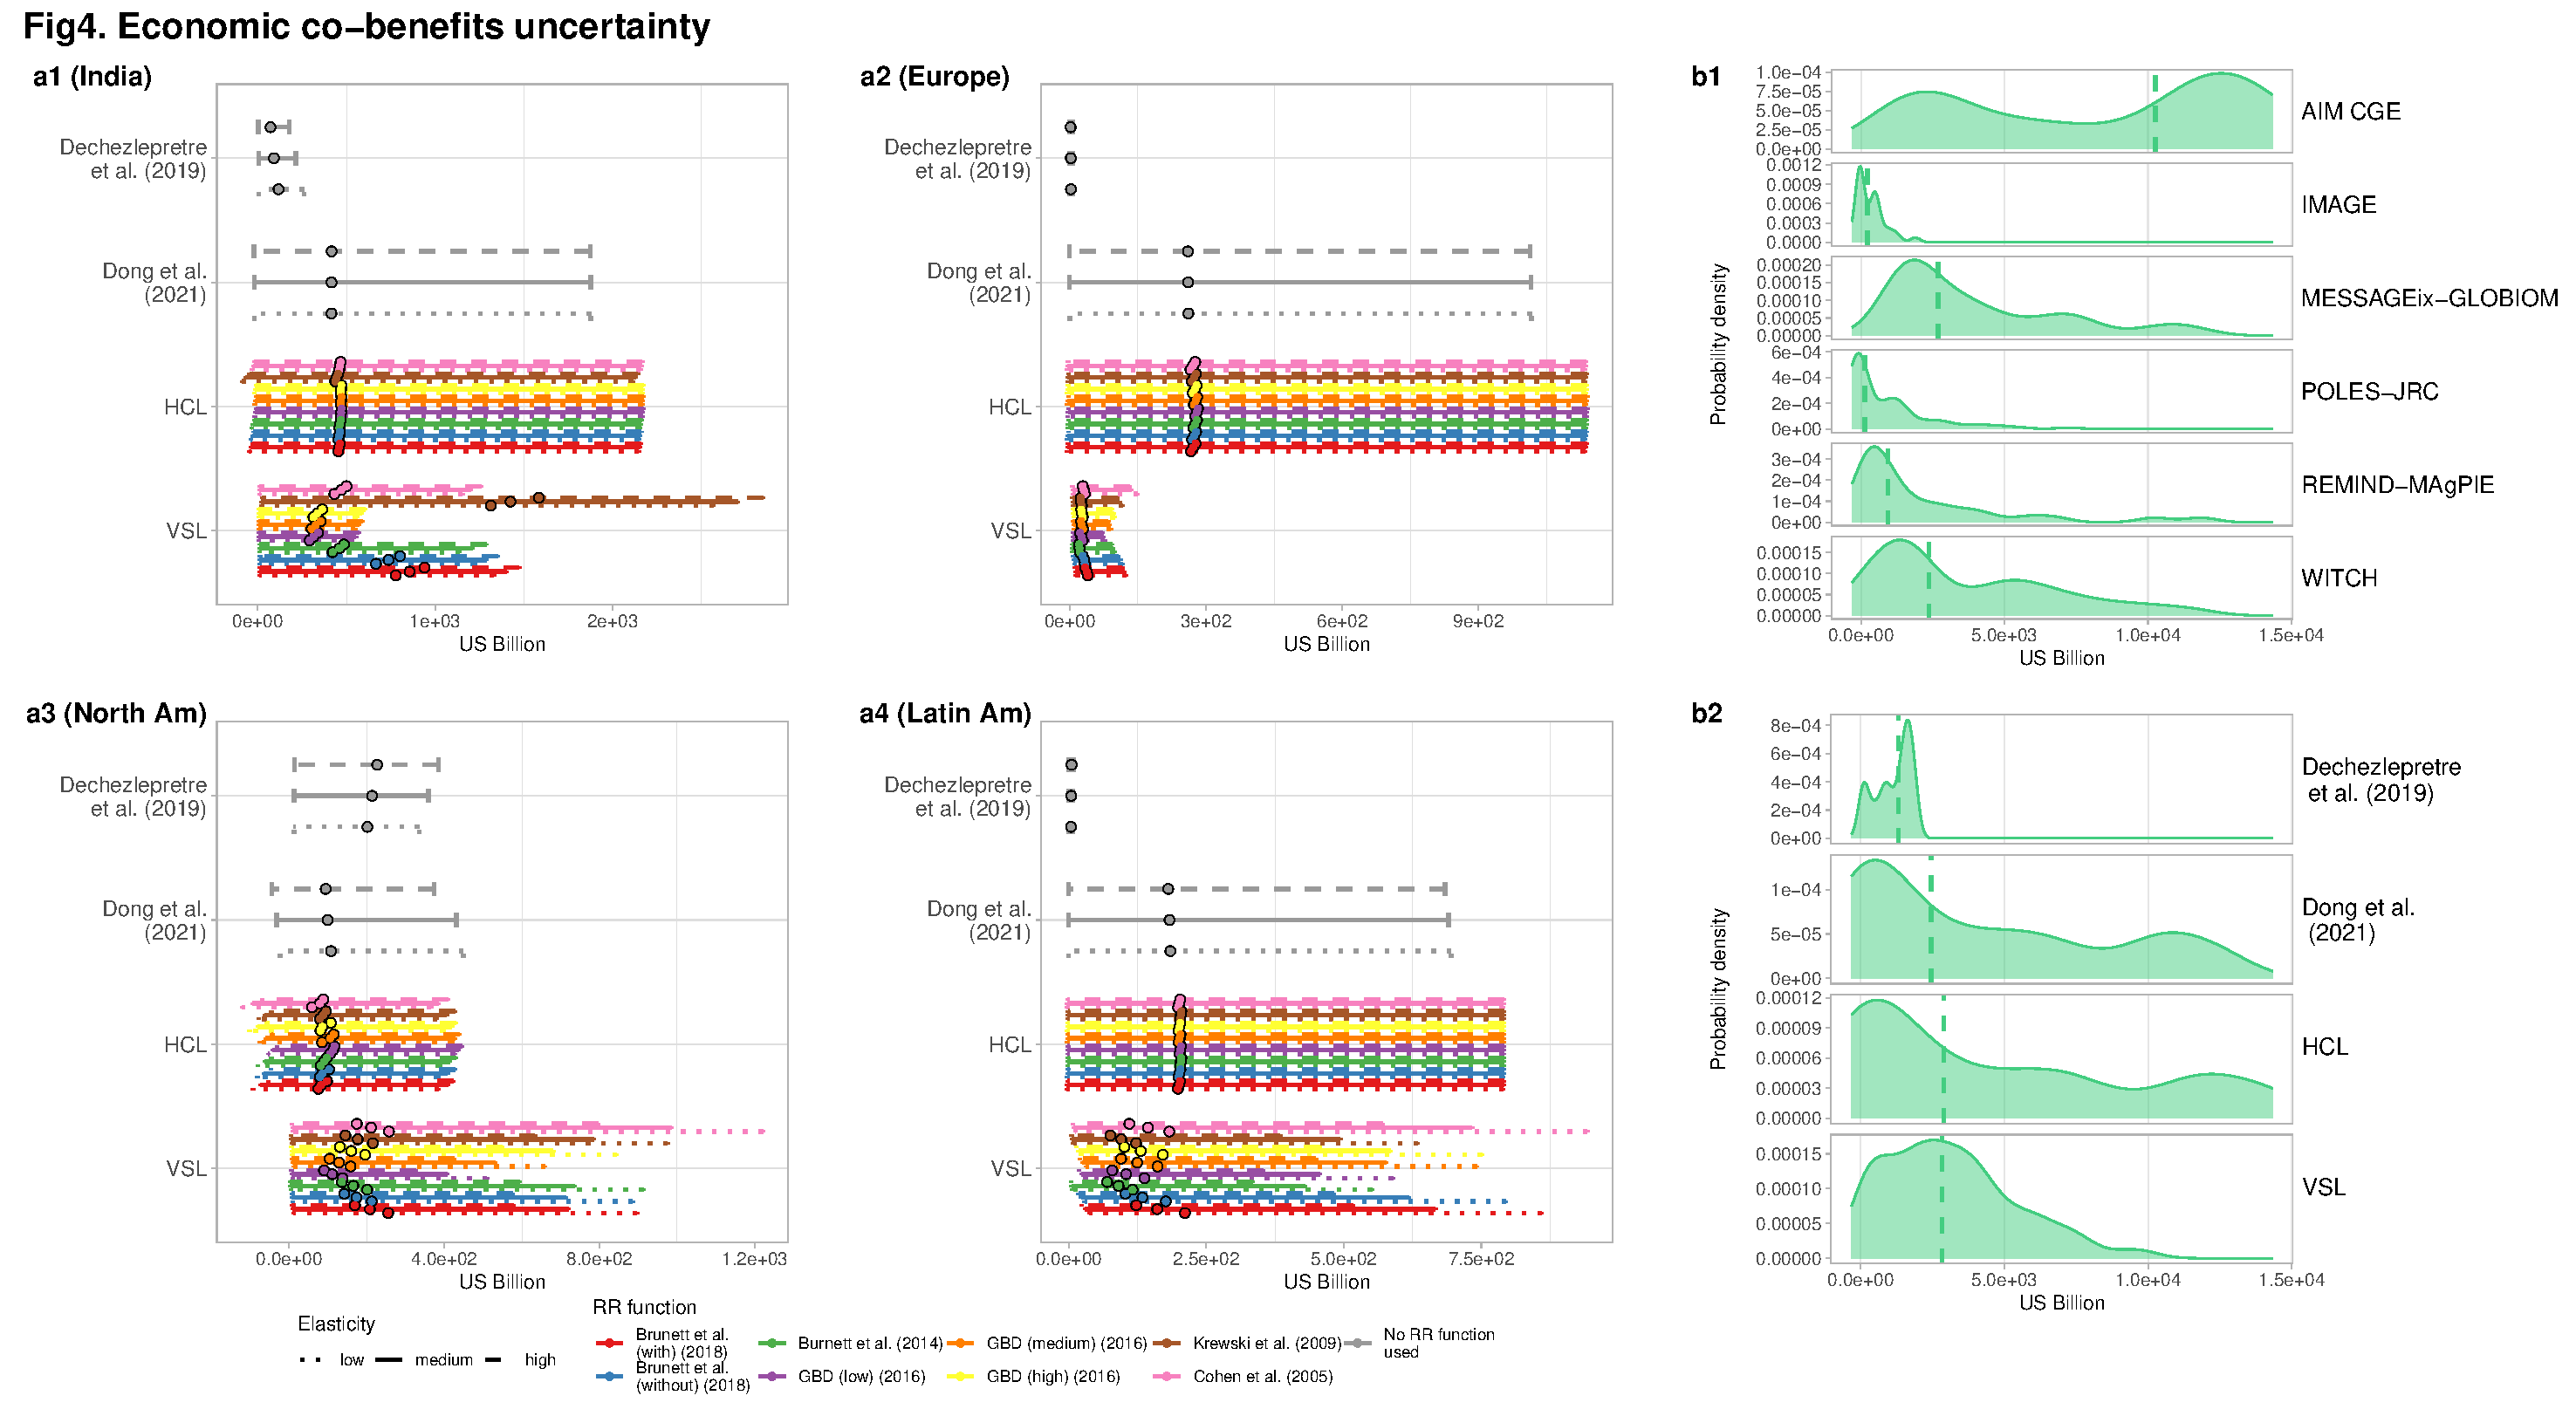
\includegraphics[width = \linewidth]{Images_statistical_meth/econ_uncertainty_2030.pdf}
    \end{figure}    
    \vfill \hfill \cite{rodes-bachs_beyond_ap}
\end{frame}


% Motivation: comparing climate policies ------------------------------------------------

\begin{frame}
    \frametitle{\scalebox{0.85}{Probability distribution \& Cummulative frequency graphs}}
    \begin{figure}[htb!]
        \centering
        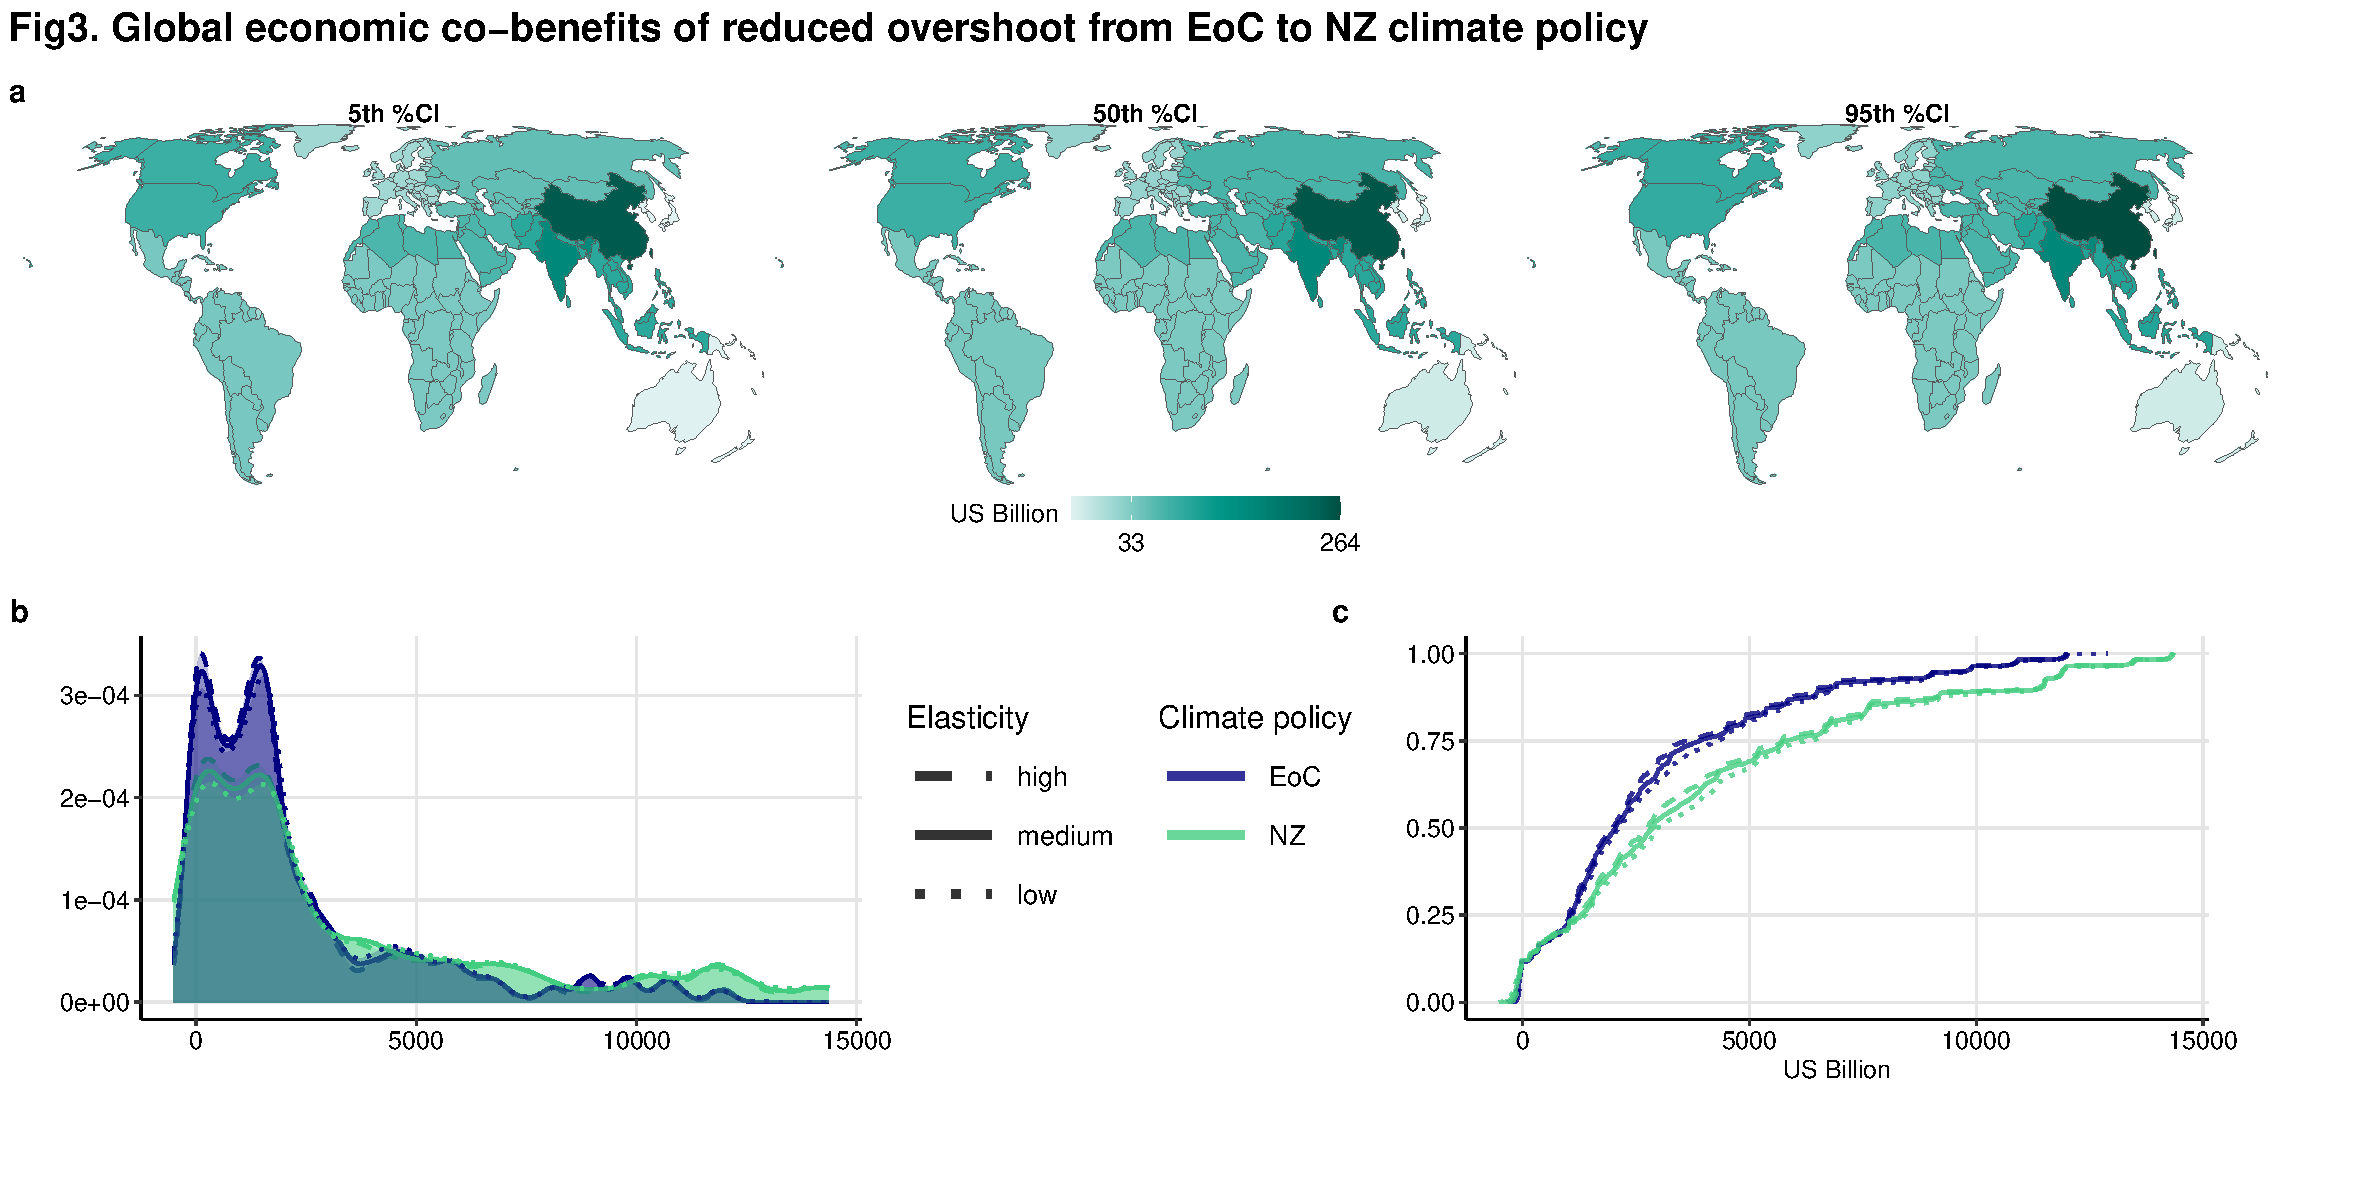
\includegraphics[width = \linewidth]{Images_statistical_meth/econ_cobenefits_2030.pdf}
    \end{figure}    
    \vfill \hfill \tiny{\cite{rodes-bachs_beyond_ap}}
\end{frame}
\begin{frame}
    \frametitle{\scalebox{0.85}{Probability distribution \& Cummulative frequency graphs}}
    \begin{figure}[htb!]
        \centering
        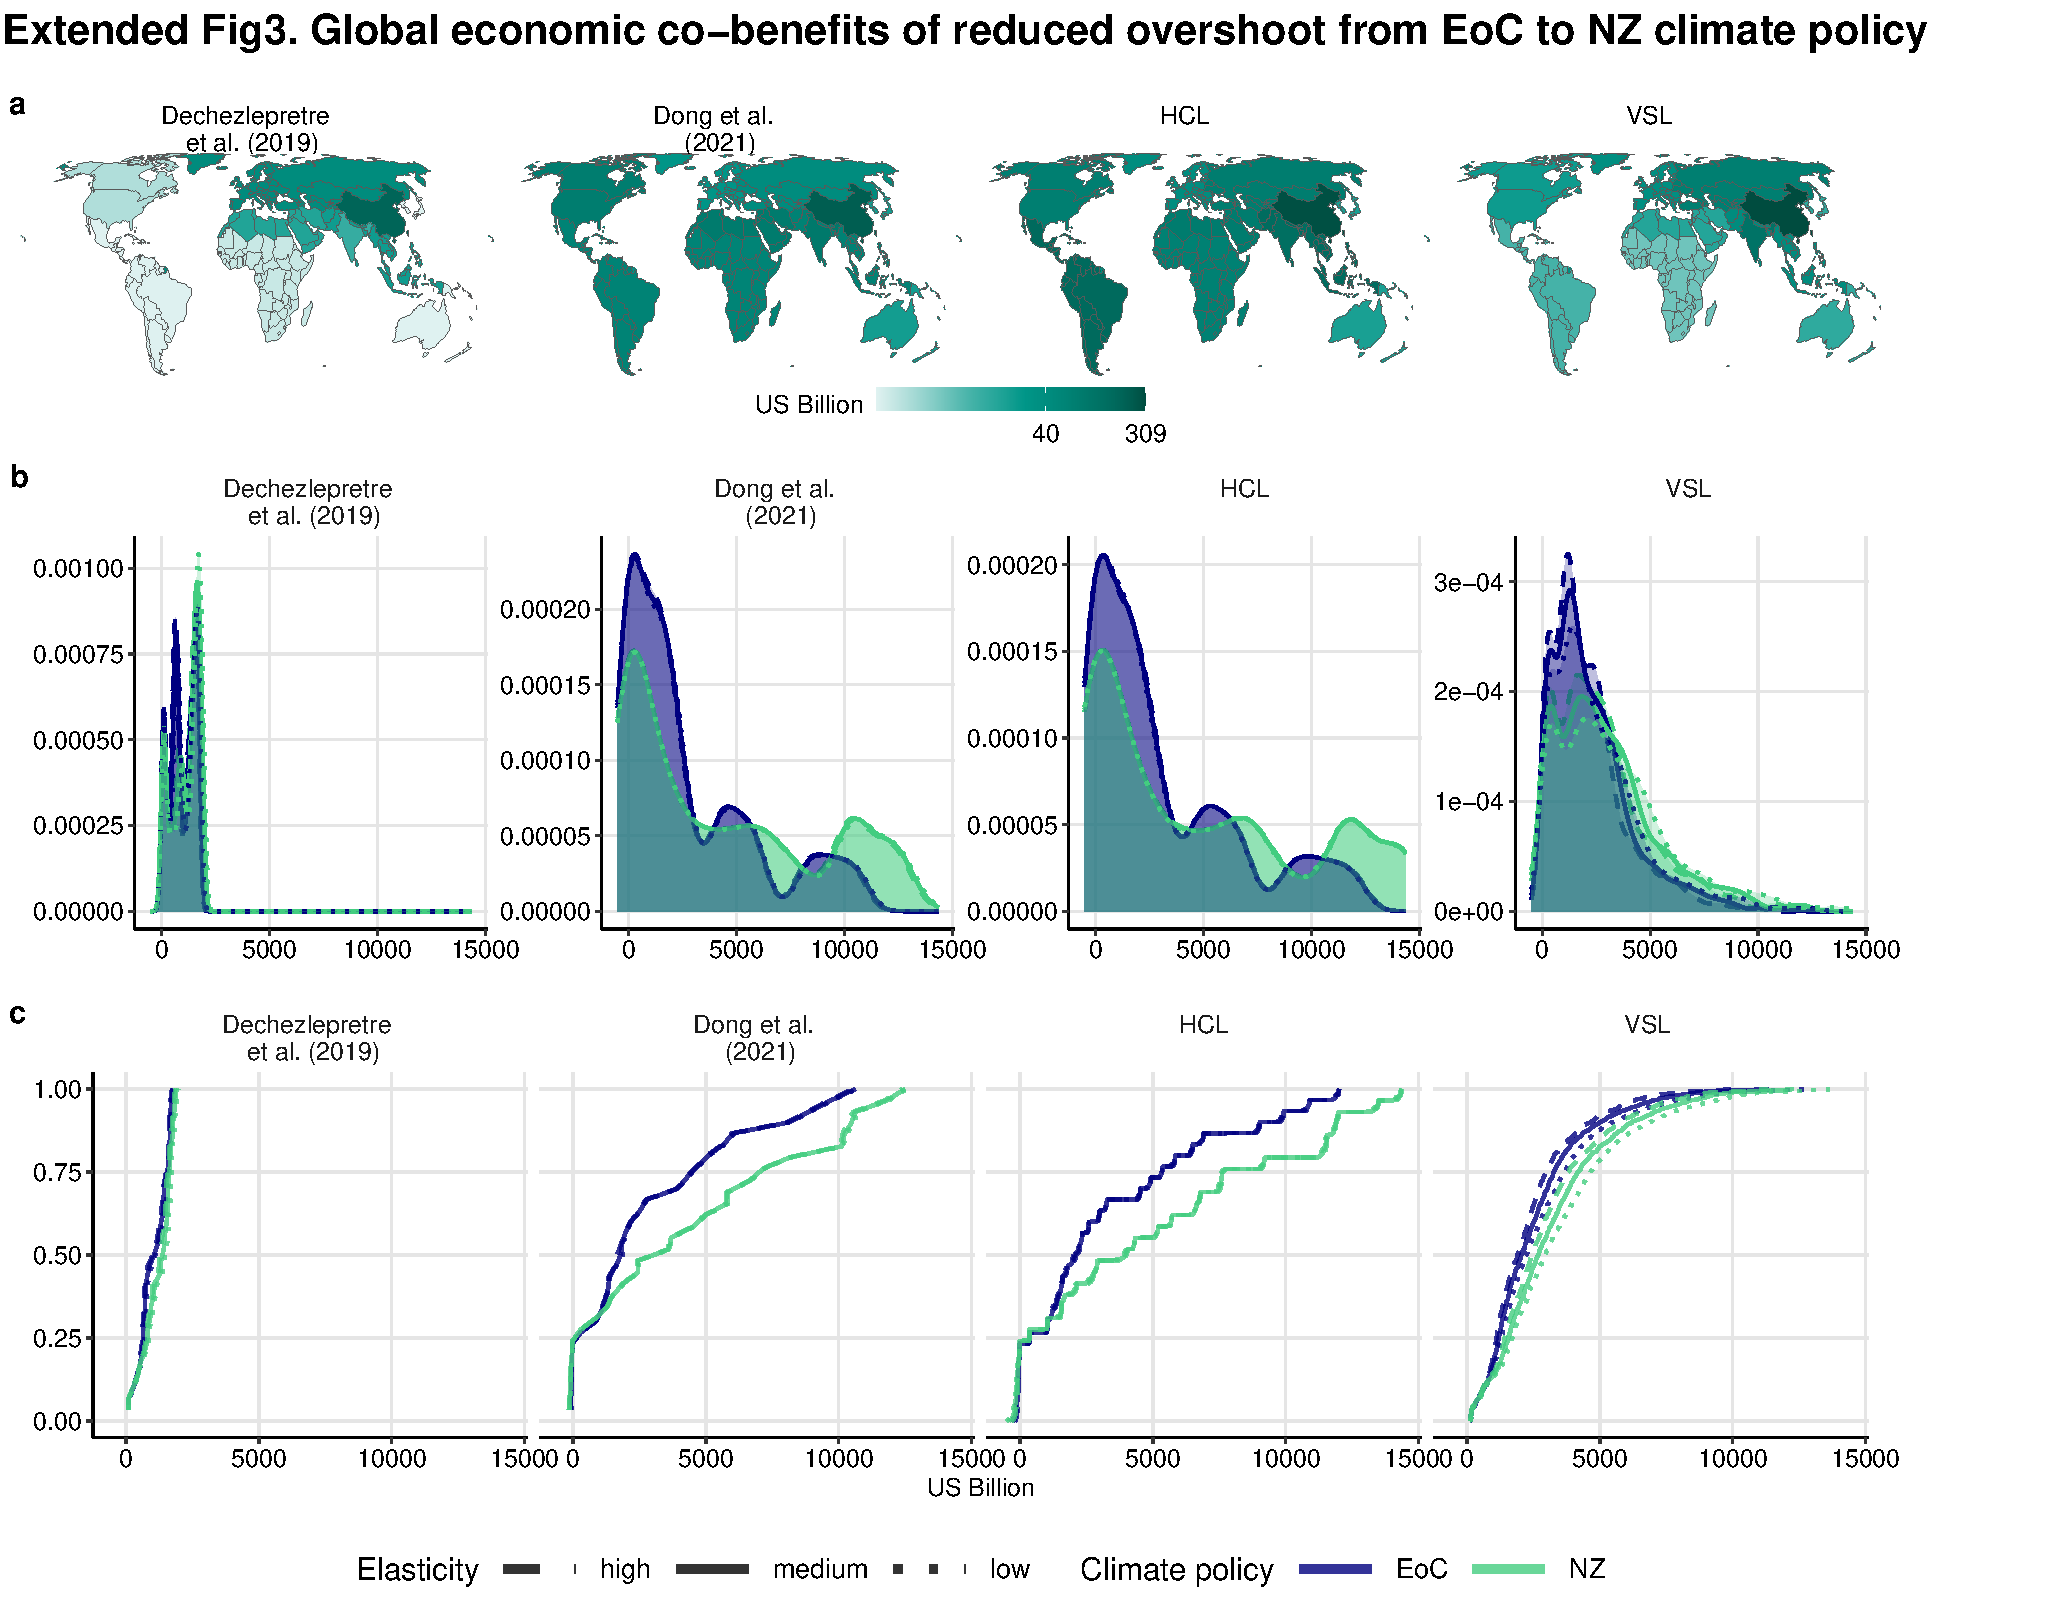
\includegraphics[width = 0.8\linewidth]{Images_statistical_meth/extended_econ_cobenefits_2030.pdf}
    \end{figure}    
    \vfill \hfill \tiny{\cite{rodes-bachs_beyond_ap}}
\end{frame}



% Binomial distribution ------------------------------------------------
\begin{frame}
    \frametitle{Binomial distribution}

    \begin{figure}
        \centering
        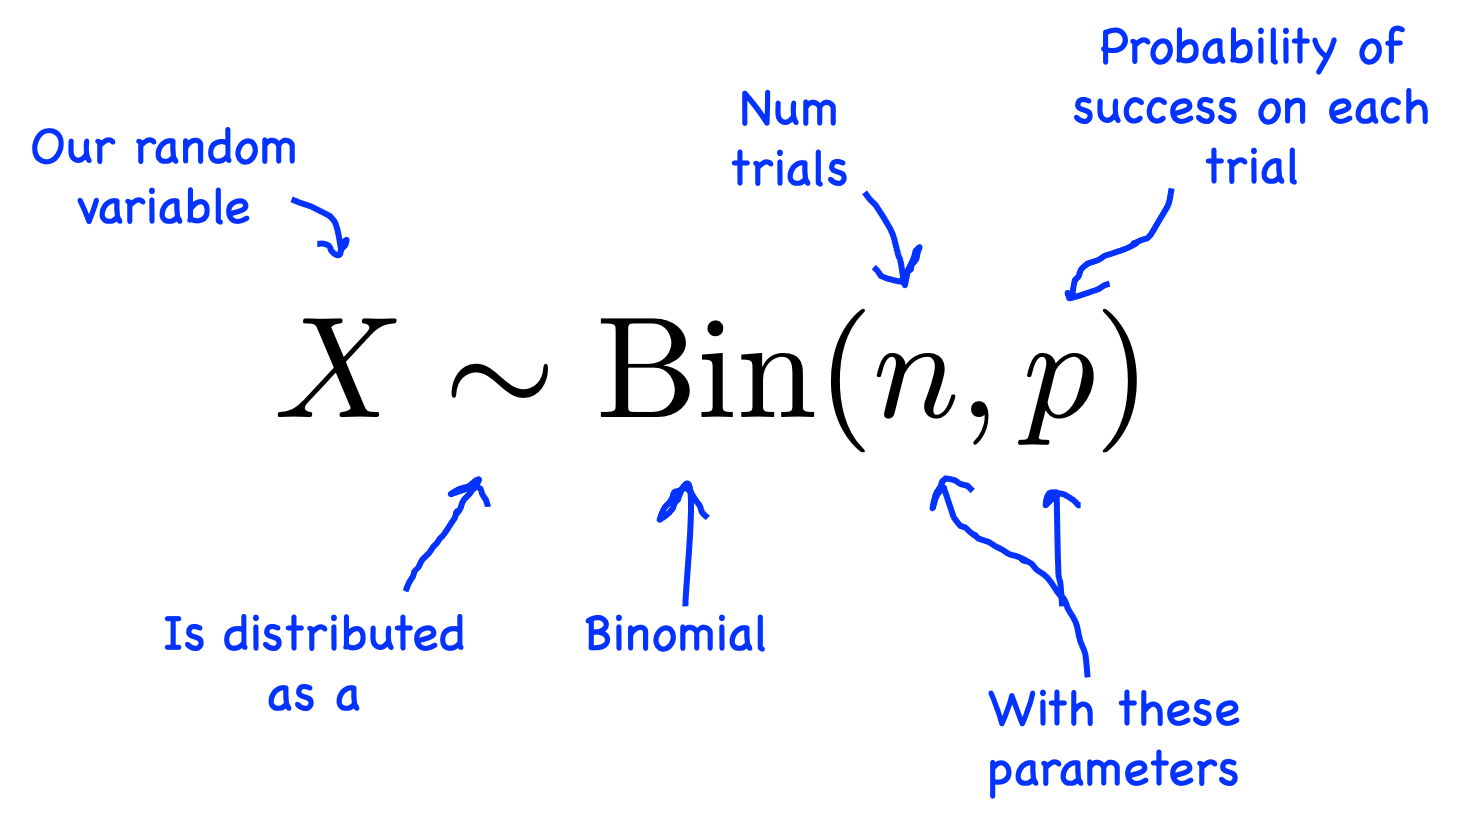
\includegraphics[width = 0.5\linewidth]{extraFigs/binomial_eq.png}
    \end{figure}
\end{frame}
\begin{frame}
    \frametitle{Binomial distribution}

    \begin{figure}
        \centering
        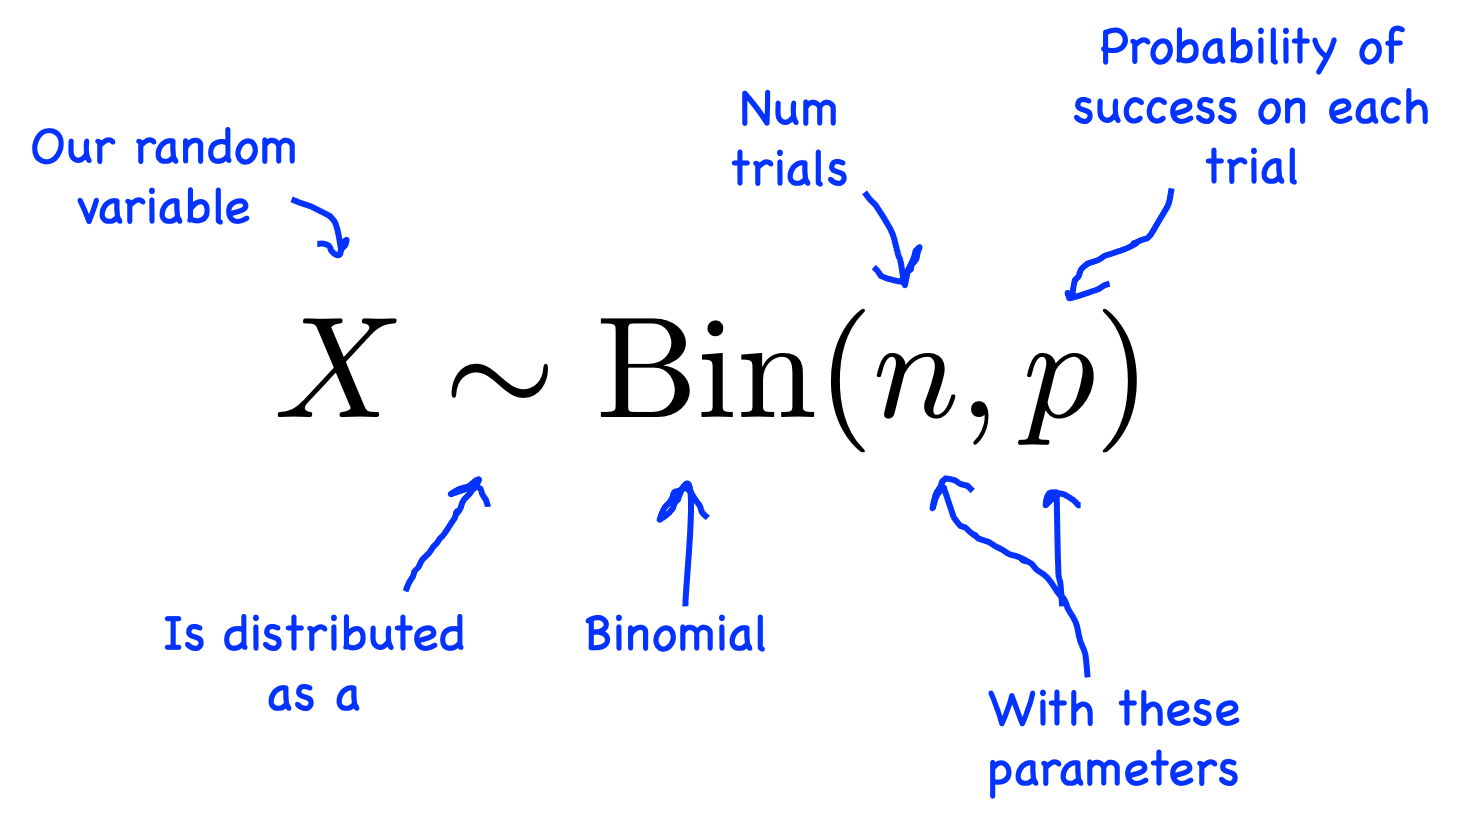
\includegraphics[width = 0.30\linewidth]{extraFigs/binomial_eq.png}
        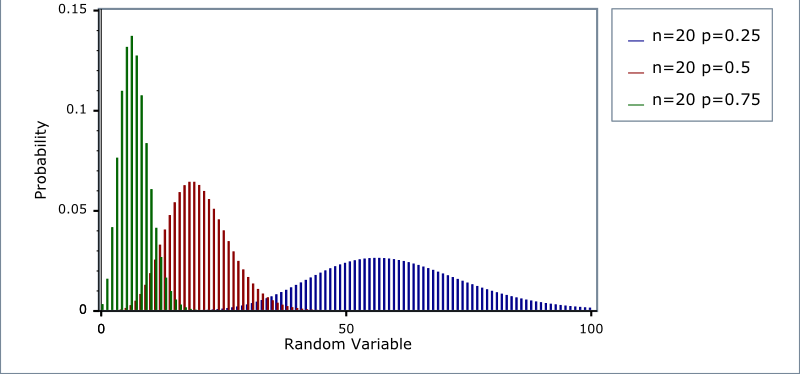
\includegraphics[width = \linewidth]{extraFigs/binomial_distrib.png}
    \end{figure}
\end{frame}

% Heavy tails ------------------------------------------------
\begin{frame}
    \frametitle{Heavy Tails}
    % There is no unique definition of a heavy-tailed distribution. Indeed, this notion only makes sense in the context of each considered model.
    % What we usually expect when we talk about heavy-tailed phenomena is some kind of different qualitative behavior of the underlying model, i.e.,
    % some deviation from the ``normal behavior'' which is caused by the extremes of the sample~\cite{Bryson1974}. Precisely because of that, 
    % heavy-tailed distributions tend to have many outliers with very high values. The heavier the tail, the larger the probability to have one 
    % or more disproportionate values in a sample; and in our case, the larger probability of high mortality outcomes.

    % Although it does not exist a universal definition, there is a general consensus and acceptance of the following one:
    \begin{alertblock}{Definition: heavy-tailed probability distribution, \cite{foss_heavy-tailed_2013}}
        A probability distribution $F(x)$ is heavy-tailed if and only if
        \begin{equation*}
            \int_\R e^{\lambda x} F(x) dx = \infty, \ \forall \lambda > 0.
        \end{equation*}    
    \end{alertblock}
    % Intuitively, a probability distribution is called heavy-tailed if it has a tail that’s
    % heavier than an exponential distribution [4]. In other words, a distribution that is
    % heavy-tailed goes to zero slower than one with exponential tails. On the contrary,
    % if a function is light-tailed, it goes to zero quicker than one with exponential tails.
    \pause{
    Intuitively:
    \begin{figure}[htb!]
        \centering
        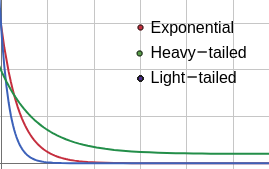
\includegraphics[width = 0.5\linewidth]{Images_statistical_meth/Tail.png}
    \end{figure}
    }  
\end{frame}
\begin{frame}
    \frametitle{Outliers analysis}
    One way of measuring the tail heaviness is computing the \textbf{tail index} [\cite{haan_extreme_2006}]\pause, \textcolor{myred}{but you required a lot of estimates.}

    \vspace{0.5cm}
    \pause{We can relay on a finite sample argument relative to the binomial random behavior of threshold exceedances.}
\end{frame}
\begin{frame}
    \frametitle{Outliers analysis}
    Consider the sequence of economic damage for a given region and year: 
    \[ X_t^1, X_t^2, X_t^3, ..., X_t^n, \; t \in \{2020, 2030 ...\} \]
    \pause Consider a \textit{high} thereshold $h$ given by the $90^{th}$ percentile of the economic damages of that region

    \pause Consider the probability of exceeding the thereshold value $h$:
    \[ p = P(X_t^i > h) \; \forall i \in \{1,...,n\}\]
    \pause Assume that this are observations from independent random variables. Thus,
    \[ \sum_{i = 1}^n \mathbbm{1}\left( X_t^{(i)} > h\right) \sim \text{Bin}(n,p) \] 
    i.e., the number of exceedances on $n$ trials follows a binomial distribution with success probability $p$.
    % This probability provides an indication of the heaviness of
    % the tail distribution. In particular, as p increases, fatter is the distribution’s tail.
    % Although with this procedure we can not obtain a precise indication of the tail
    % heaviness, we do identify the distribution with the heavier tail, which fits exactly
    % our analysis aim
\end{frame}
\begin{frame}
    \frametitle{Outliers analysis}
    \begin{figure}[htb!]
        \centering
        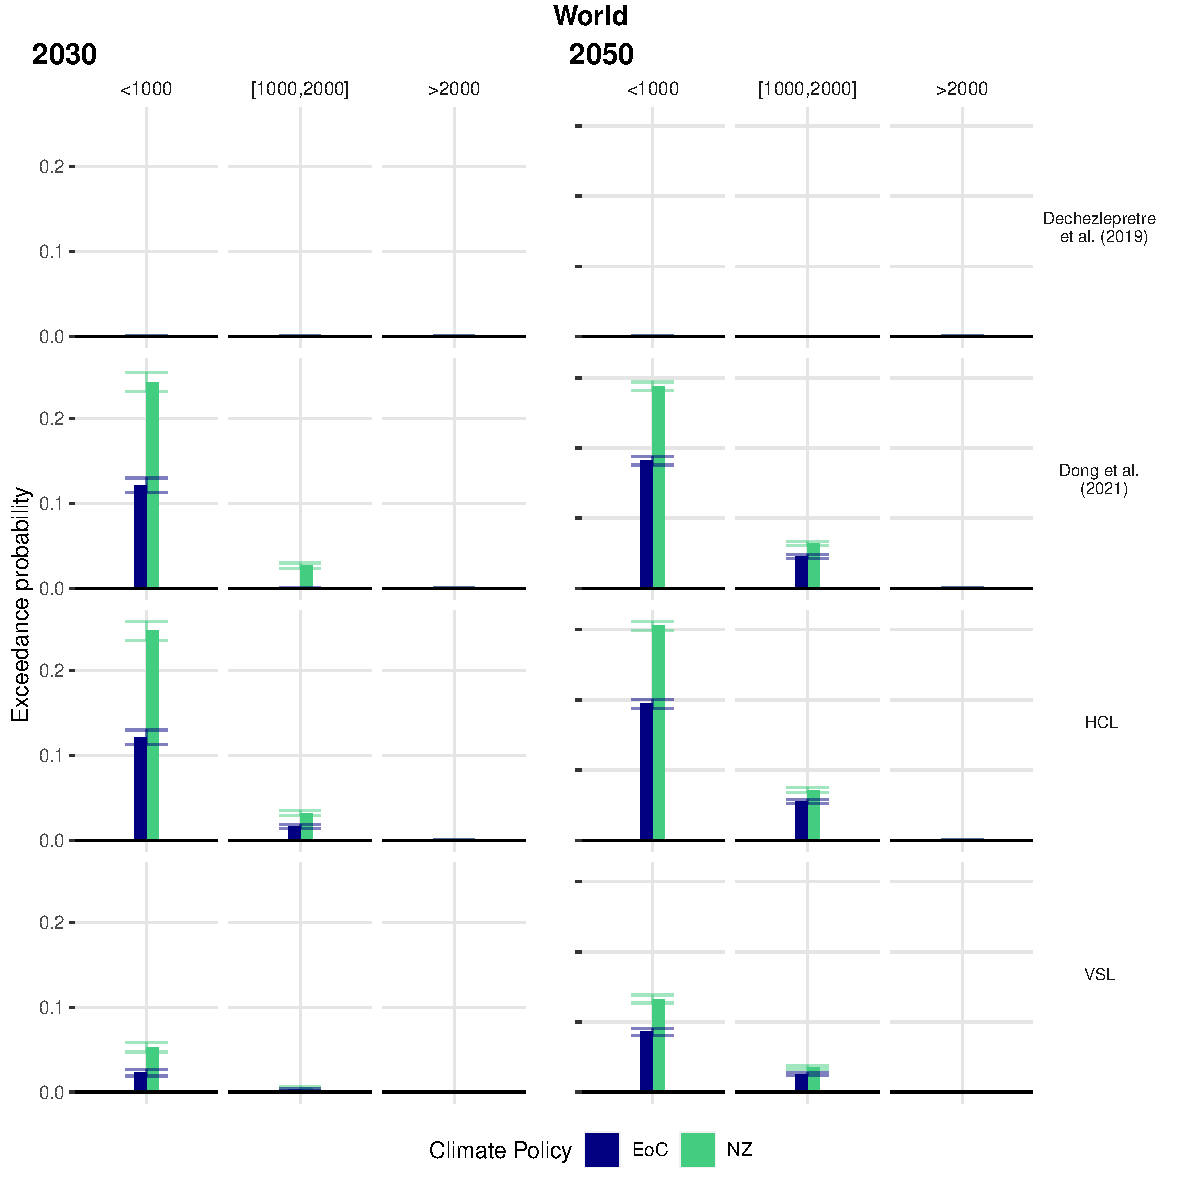
\includegraphics[width = 0.6\linewidth]{Images_statistical_meth/tail_heaviness_WORLD.pdf}
    \end{figure}    
    \vfill \hfill \tiny{\cite{rodes-bachs_beyond_ap}}
\end{frame}


% Kolmogorov-Smirnov test ------------------------------------------------
\begin{frame}
    \frametitle{Kolmogorov-Smirnov test}
    % We consider the Kolmogorov-Smirnov two-sample test, which is an adaptation
    % of the non-parametric Kolmogorov-Smirnov one-sample test. It compares the
    % empirical distribution function of two samples. Intuitively, the test answers the
    % question “What is the probability that these two sets of samples were drawn from
    % the same (but unknown) probability distribution?”
    Consider two distribution functions.

    \vspace{0.5cm}
    \pause Intuitively, the test answers: ``What is the probability that these two sets of samples were drawn from
    the same (but unknown) probability distribution?''
    
    \vspace{0.5cm}
    \pause
    In a more formal way:
    \[
    \left\{\begin{array}{ll}
        H_0: & F_X(x) = F_Y(x) \ \  \forall x, \\
        H_1: & F_X(x) \neq F_Y(x) \ \ \text{for some }x
    \end{array}\right.
    \]
    \pause
    which is equivalent to
    \[
    \left\{\begin{array}{ll}
        H_0: & \scalebox{0.95}{\text{NZ and EoC climate policies have the \textbf{same} distribution function},} \\
        H_1: & \scalebox{0.95}{\text{NZ and EoC climate policies have the \textbf{different} distribution function}}
    \end{array}\right.
    \]
\end{frame}

\begin{frame}
    \frametitle{Kolmogorov-Smirnov test}
    \begin{figure}[htb!]
        \centering
        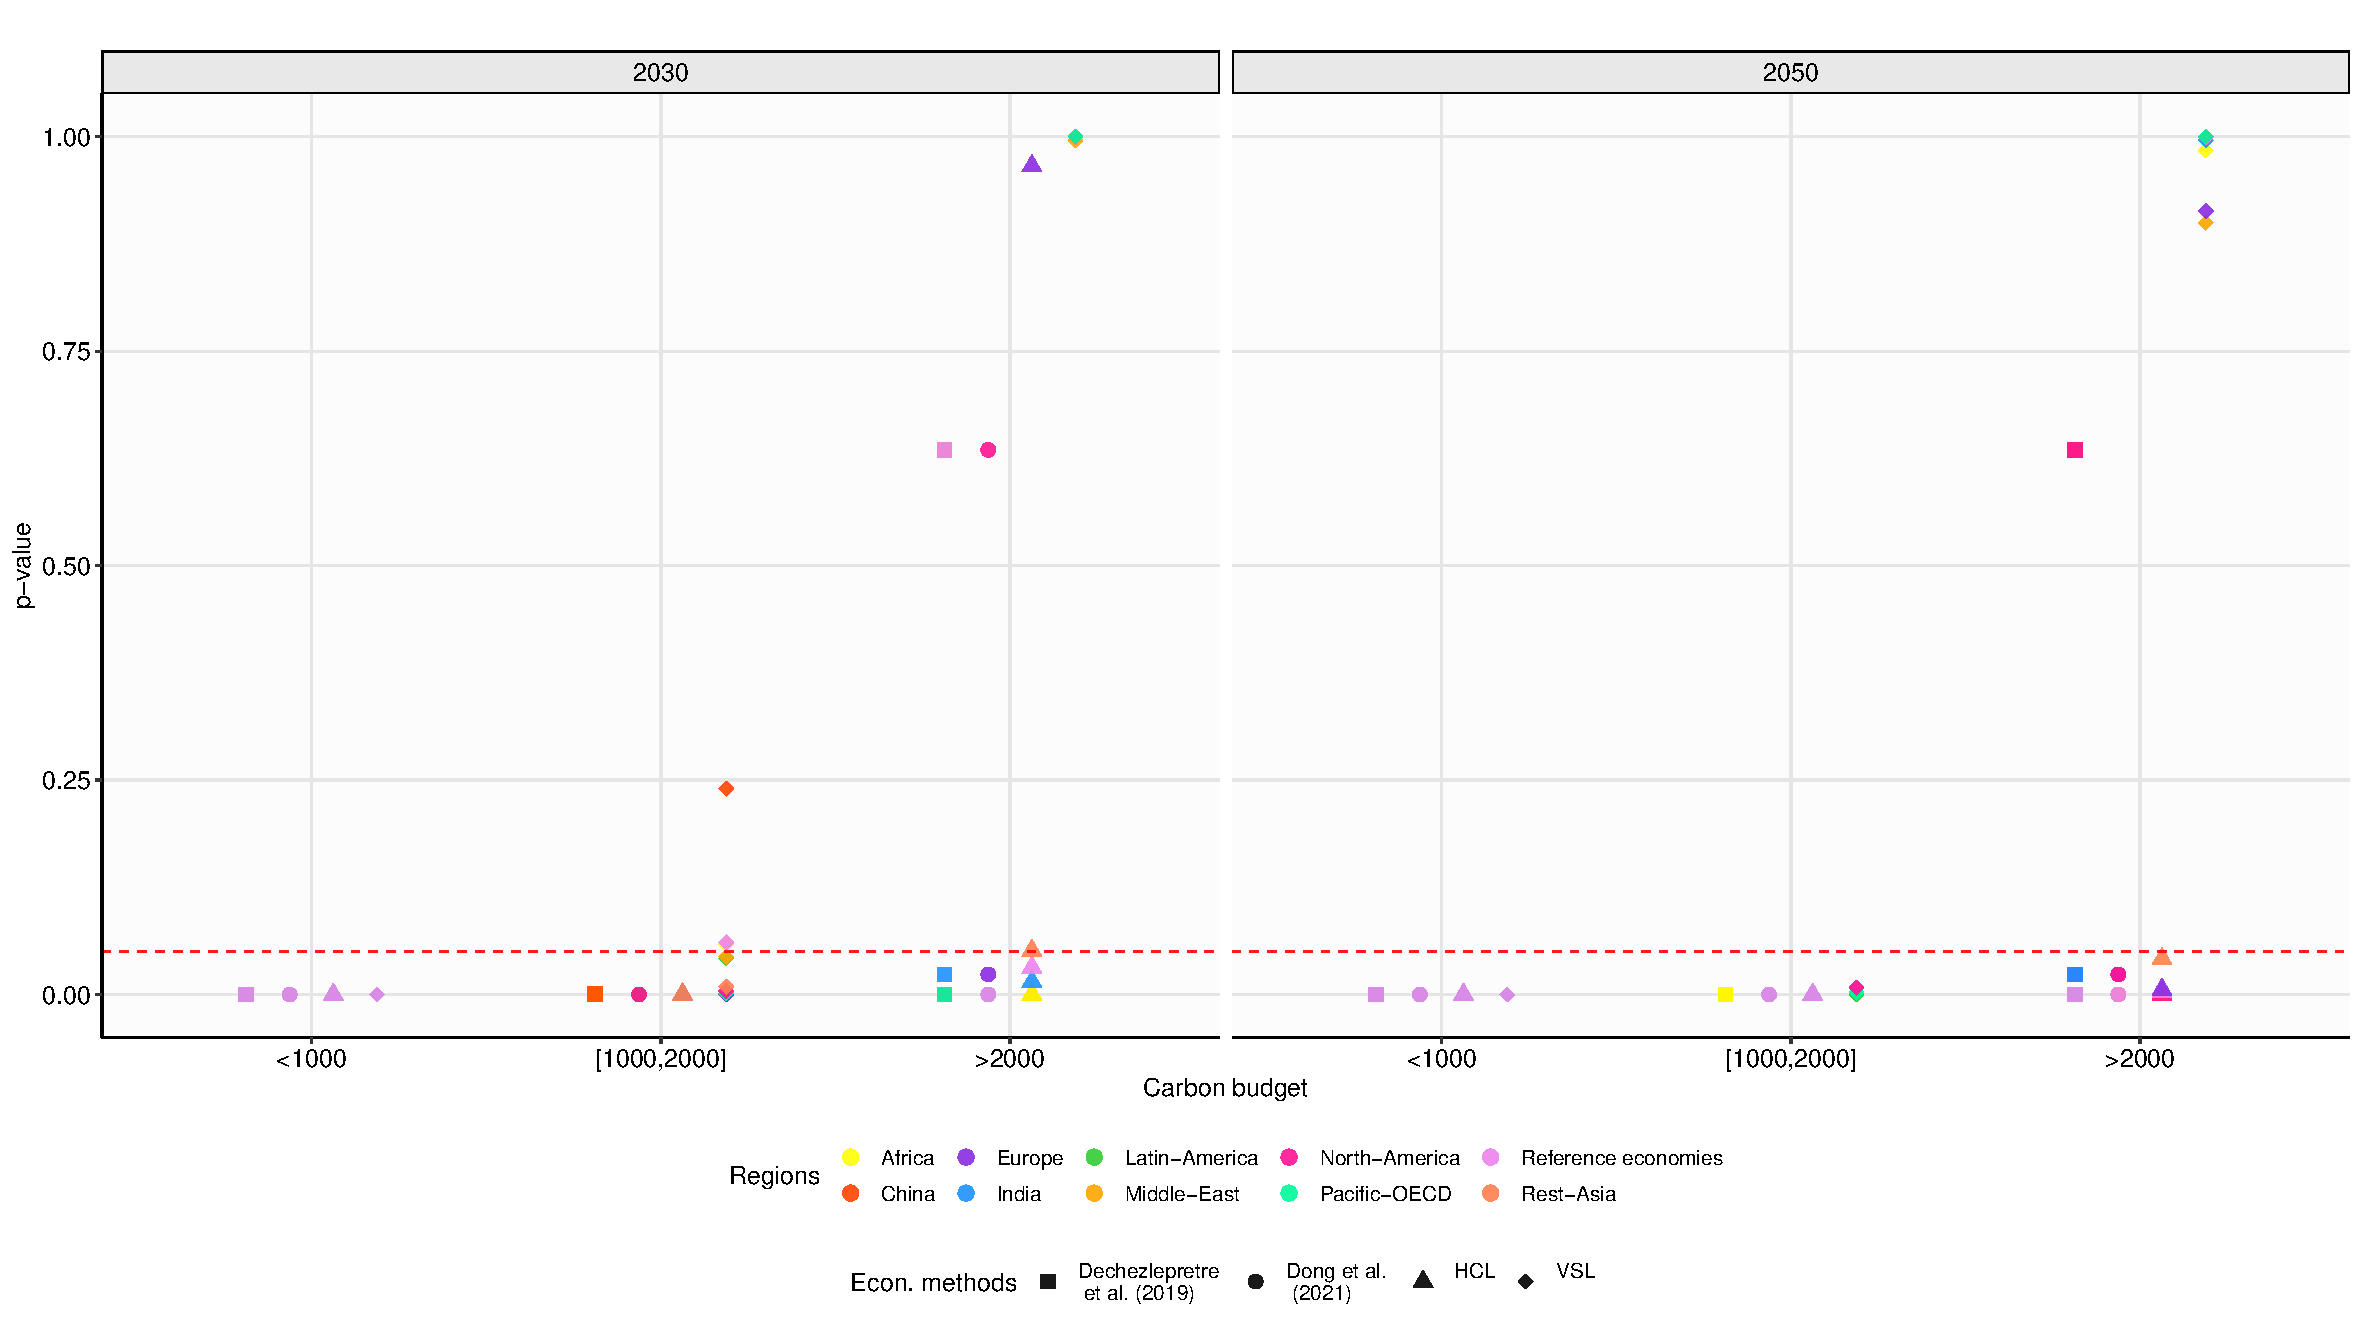
\includegraphics[width = 0.98\linewidth]{Images_statistical_meth/ks_econ_2030_2050.pdf}
    \end{figure}    
    \vfill \hfill \tiny{\cite{rodes-bachs_beyond_ap}}
\end{frame}
